\documentclass{article}
\usepackage[margin=1in]{geometry}
\usepackage{../common}
\usepackage{../pagesetup}

\begin{document}
%\lecture{**LECTURE-NUMBER**}{**DATE**}{**LECTURER**}{**SCRIBE**}
\lecture{20}{November 15}{Sasha Rush}{Shangyan Li, Alex Wu, Nicol\`o Foppiani, Kevin Liu, Daniel Merchan, Milan Ravenell}{Importance Sampling and Particle Filtering}%% Add your scribe names!!

\subsection{State space models and Kalman Filter}

\subsubsection{Introduction on state space models}
The first topic which has been covered during this lecture is a review about state space models and Kalman Filter.
A state space model (SSM) is a Hidden Markov Model (HMM) with continuous hidden states.
%add graph


\begin{center}
\begin{tikzpicture}
\node[latent] (x_1) at  (0,0) {$x_1$};
\node[latent] (x_2) at  (3,0) {$x_2$};
\node[latent] (x_3) at  (6,0) {$x_3$};

\node[latent] (x_t) at  (11,0) {$x_t$};

\node[latent] (z_1) at  (0,3) {$z_1$};
\node[latent] (z_2) at  (3,3) {$z_2$};
\node[latent] (z_3) at  (6,3) {$z_3$};

\node[latent] (z_t) at  (11,3) {$z_t$};

\path (x_3) to node {\dots} (x_t);
\path (z_3) to node {\dots} (z_t);

\edge {z_1} {x_1};
\edge {z_2} {x_2};
\edge {z_3} {x_3};
\edge {z_t} {x_t};

\edge {z_1} {z_2};
\edge {z_2} {z_3};

\end{tikzpicture}
\end{center}


The model is specified by
\[z_t = g_t(z_{t-1}, \epsilon_t)\]
\[x_t = h_t(z_t, \delta_t)\]
where $\epsilon$ and $\delta$ represent a noise which is added in the transition between two states. $z_t$ is usually referred as the transition model and $x_t$ as the observation model. 

An important case is where the transition functions are linear-Gaussian, which means:
\[z_t = A_t(z_{t-1} + \epsilon_t) \text{ where } \epsilon_t \sim \mathcal{N}(0, Q_t)\]
\[x_t = C_t z_t + \delta_t \text{ where } \delta_t \sim \mathcal{N}(0, R_t)\]

This case is called linear-Gaussian SSM (LG-SSM) or linear dynamical system (LDS).

In most situations we can assume that the process is stationary and considering the model functions independent of time label.

In principle this problem can be solved with the architecture developed for graphical models: this is a directed graphical model in which each variables is Gaussian distributed. Thus the whole model can be solved raising to a multivariate Gaussian for the whole model.\\
However this model is historically relevant and thus deserves a proper study.

\subsubsection{Kalman Filter}
In fact, if we know that $p(z_1)$ is MVN, then $p(z_t|x_{1:t})$ will be MVN.
Suppose now to have observed $x_{1:t}$ and we want to compute $p(z_t|x_{1:t})$.

\begin{center}
\begin{tikzpicture}
\node[latent, shade] (x_1) at  (0,0) {$x_1$};
\node[latent, shade] (x_2) at  (3,0) {$x_2$};
\node[latent, shade] (x_3) at  (6,0) {$x_3$};

\node[latent, shade] (x_t) at  (11,0) {$x_t$};

\node[latent] (z_1) at  (0,3) {$z_1$};
\node[latent] (z_2) at  (3,3) {$z_2$};
\node[latent] (z_3) at  (6,3) {$z_3$};

\node[latent] (z_t) at  (11,3) {$z_t$};

\path (x_3) to node {\dots} (x_t);
\path (z_3) to node {\dots} (z_t);

\edge {z_1} {x_1};
\edge {z_2} {x_2};
\edge {z_3} {x_3};
\edge {z_t} {x_t};

\edge {z_1} {z_2};
\edge {z_2} {z_3};

\end{tikzpicture}
\end{center}

We can marginalize, obtaining a tree, on which we can apply exact belief propagation (BP).

\begin{center}
\begin{tikzpicture}
\node[latent] (z_1) at  (0,3) {$z_1$};
\node[latent] (z_2) at  (3,3) {$z_2$};
\node[latent] (z_3) at  (6,3) {$z_3$};

\node[latent] (z_t) at  (11,3) {$z_t$};

\path (z_3) to node {\dots} (z_t);

\edge {z_1} {z_2};
\edge {z_2} {z_3};

\end{tikzpicture}
\end{center}

There is a difference with exact belief propagation in the discrete case:
\begin{itemize}
    \item discrete: Bel($z_t$) is an array
    \item MVN: Bel($z_t$) is MVN with $\vec{\mu}$ and $\Sigma$
\end{itemize}

The inference algorithm based on MVN BP in this case is called \textbf{Kalman filter}. 
This is a crucial and popular algorithm, central to multiple technologies. However, at its core, it just runs the LG formula multiple times as part of BP. 

\subsubsection{Example: LG-SSM for tracking application}

We have an object moving in the 2-D plane: the hidden state represents the position and velocity at every timestep, and the observed state is the observed position at the every timestep.

\begin{center}
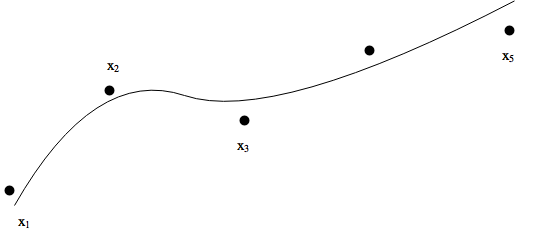
\includegraphics[width=0.8\textwidth]{Drawing_kalman_filter.png}
\end{center}

\[ \vec{z_t} = [ z_{1, t},~z_{2, t},~\dot{z}_{1, t},~\dot{z}_{2, t}] \]
$A_t$ updates $z_t \rightarrow z_{t+1}$\\
$C_t$ generates $x_t$ given $z_t$: in this case it sets $x_{1, t} = z_{1, t}$ and $x_{2, t} = z_{2, t}$\\
$\epsilon_t$ represents the noise related to physics\\
$\delta_t$ represents the noise generated by the sensors in the observations\\

\subsubsection{Kalman smoothing}
Suppose we observed $x_{1:T}$ and we want to infer $z_t$. We can use another variant of BP in which we combine the messages from the past and from the future: this is called \textbf{Kalman smoothing}.


\subsection{Review on importance sampling}


\subsubsection{Basic Idea}
We aim to sample form $p$ to approximate $f(z)$ using MonteCarlo sampling:
\begin{center}
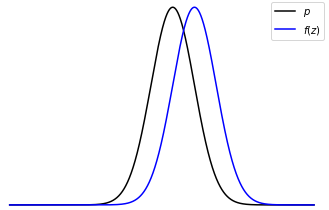
\includegraphics[scale=0.5]{normal_dist.png}
\end{center}

To approximate integrals of the form:
\[ \mathbb{E}_p[f(z)] = \int q(z) \frac{p(z)}{q(z)}f(z)dz \approx \frac{1}{S} \sum_{i=1}^S\frac{p(z^s)}{q(z^s)}f(z^s) = \sum_{i=1}^Sw^sf(z^s)\]
$w^s = \frac{p(z^s)}{q(z^s)}$ are importance weights associated with each sample.

\subsubsection{Unnormalized Distributions}
Frequently will have unnormalized target distribution $\tilde{p}(z)$ but not its normalization constant $Z_p$. Similarly, may have unnormalized proposal $\tilde{q}(z)$ and its unknown normalization constant $Z_q$.
\[p(z) = \frac{\tilde{p}(z)}{Z_p} \text{ and } q(z) = \frac{\tilde{q}(z)}{Z_q}\]
Substituting into the desired expectation:
\[ \mathbb{E}_p[f(z)] = \frac{Z_q}{Z_p} \int q(z) \frac{\tilde{p}(z)}{\tilde{q}(z)}f(z)dz \approx \frac{Z_q}{Z_p}\frac{1}{S} \sum_{i=1}^S \tilde{w}^sf(z^s)\]
where $\bar{w}_s = \frac{\bar{p}(z^s)}{\bar{q}(z^s)}$.

Now, how to compute $\frac{Z_q}{Z_p}$? Can also importance sample from $q$.
\[\frac{Z_p}{Z_q} = \frac{1}{Z_q}\int\tilde{p}(z)dz = \frac{1}{Z_q}\int q(z)\frac{\tilde{p}(z)}{q(z)}dz = \int q(z)\frac{\tilde{p}(z)}{\tilde{q}(z)}dz \approx \frac{1}{S}\sum_{i=1}^S\tilde{w}^s\]
Substituting the sampled $\frac{Z_p}{Z_q}$ back:
\[\mathbb{E}_p[f(z)] \approx \sum_{s=1}^S \frac{\tilde{w}^s}{\sum_{s'}\tilde{w}^{s'}}f(z^s) = \sum_{s=1}^S w^s f(z^s)\]

\textbf{Note}: This form of importance sampling is convenient as it lets us work with unnormalized distributions. However, in many cases is much less convenient than, for instance, rejection sampling or MonterCarlo sampling because it is not fully clear how to use the weights. 


Now consider getting samples from $p$. We need to define $p(x)$ in terms of $\mathbb{E}_p[f(x)]$ using a $\delta$ function that returns $1$ if it's the value we want, $0$ otherwise:

\[p(x=x') = \mathbb{E}_p[\delta_{x'}(x)]\]
Then, our estimate in terms of importance sampling is:
\[p(x) = \sum_{s=1}^S w_s \delta_{x^s}(x)\]

But we actually want unweighted samples, which can be obtained through \textbf{re-sampling}: pick $x^s$ with probability $w^s$. In other words, we create a discrete set that approximates the original distribution and then we draw samples from that discrete set based on a categorical distribution weighted by the $w_s$. 

\subsubsection{Example} Recall from last class, we have:
\begin{align*}
    p(\theta | Data) &= \frac{p(Data|\theta)p(\theta)}{p(Data)} \\
    \tilde{p}(\theta | Data) &= p(Data|\theta)p(\theta) \\
\end{align*}

Notice we drop the normalization term for $\tilde{p}$. Then $q(\theta) = p(\theta)$, which implies that we importance-sample based on the prior. This gives normalized $w_s$:
\[
w_s = \frac{\tilde{p}(\theta_s)/{q}(\theta_s)}{\sum_{s'} \tilde{p}(\theta_s)/{q}(\theta_s)} =\frac{p(Data| \theta_s)}{\sum_{s'} p(Data|\theta_{s'}) }
\]

In summary, we run importance-sampling to compute the posterior of the parameters by sampling different parameters from the priors and then by assigning weights to each of those different parameters based on likelihood in the data. The resulting samples are unbisased samples from the distribution of interest. 


\subsection{Particle Filtering/Sequential Monte Carlo}
There might be cases of space-state models in which it might not be possible to derive closed-form expressions based on LG for the update equations. In those cases, a sampling-based approaches offer an alternative method. 

In order to approximate the belief state of an entire sequence, we can use a weighted set of particles as follows:  
\[p(z_{1:t}=z'_{1:t}|x_{1:t}) = \int p(z_1,...,z_t|x_{1:t})\delta_{z'}(z)dz \approx \sum_{s=1}^S \hat{w}_t^s \delta_{z'}(z^s_{1:t})\]
where $\hat{w}_t^s$ represents the normalized weight of sample $s$ at time $t$. \\

We update the belief state using importance sampling, with the following importance weights. 
\[w_t^s \sim \frac{p(z_{1:t}|x_{1:t})}{q(z_{1:t}|x_{1:t})}\]
The numerator can be expressed as follows: 
\[p(z_{1:t}|x_{1:t}) \propto p(z_{1:t}|x_{t-1})p(x|t|z_{1:t},y_{t-1}) \propto p(x_t|z_t)p(z_t|z_{t-1})p(z_{1:t-1}|x_{1:t})\]
where $p(x_t|z_t)$, $p(z_t|z_{t-1})$, and $p(z_{1:t-1}|x_{1:t})$ correspond to the observation, transition, and recursion of the sequence, respectively. \\

Meanwhile, we can express the denominator as
\[q(z_{1:t}|x_{1:t}) \propto q(z_t|z_{1:t-1},y_{1:t})q(z_{1:t-1}|x_{1:t-1})\]

Our importance weights, therefore, simplify to
\[w_t^s \propto \frac{p(x_t|z_t)p(z_t|z_{t-1})p(z_{1:t-1}|x_{1:t})}{q(z_t|z_{1:t-1},y_{1:t})q(z_{1:t-1}|y_{1:t-1})} = \frac{p(x_t|z_t)p(z_t|z_{t-1})}{q(z_t|z_{1:t-1},y_{1:t})}w_{t-1}^s\]

Using this expression, we have the following algorithm to approximate the belief state. \\
1. Start with particles $(w_t,z_t)^{(s)}$. \\
2. At each time step $t$ for particle $x$, calculate $w_t^s = \frac{p(x_t|z_t)p(z_t|z_{t-1})}{q(z_t|z_{1:t-1},y_{1:t})}w_{t-1}^s$ and sample $z_t^s \sim q(z_t|z^s_{1:t-1},x_t)$. \\
3. Compute $p(z_t,x_{1:t})$

\end{document}
